\documentclass[lang=cn,11pt,a4paper,cite=authornum]{paper}

\title{形式语言与自动机实验一:NFA到DFA的转化\ 实验报告}
\author{毛子恒 \and 邹宇江 \and 王敏行 \and 曾嘉伟}
\institute{北京邮电大学\ 计算机学院}

\date{\zhtoday}

% 本文档命令
\usepackage{array}
\newcommand{\ccr}[1]{\makecell{{\color{#1}\rule{1cm}{1cm}}}}
\nocite{*}

\begin{document}

\maketitle

\section*{小组成员}

\setlength{\tabcolsep}{7mm}
{
    \begin{table}[htbp]
        \centering
        \begin{tabular}{llll}
            班级:2019211309 & 姓名:毛子恒 & 学号:2019211397 & 分工:代码\ 文档 \\

            班级:2019211309 & 姓名:邹宇江 & 学号:2019211416 & 分工:测试\ 文档 \\

            班级:2019211309 & 姓名:王敏行 & 学号:2019211410 & 分工:测试\ 文档 \\

            班级:2019211309 & 姓名:曾嘉伟 & 学号:2019211396 & 分工:测试\ 文档 \\
        \end{tabular}
    \end{table}
}

\tableofcontents
\newpage

\section{需求分析}

\subsection{题目描述}

输入一个NFA,输出等价转化出的DFA。

\subsection{输入描述}

程序从标准输入中读入数据。

以下描述中\textbf{字符串}均特指不包含空格、回车等特殊字符的ASCII字符序列。\textbf{要求输入是一个合法的NFA}。

第一行输入若干字符串,用空格分隔,表示NFA的状态集合,\textbf{要求输入不出现重复状态},设集合大小为$n$。

第二行输入若干字符串,用空格分隔,表示NFA的字母表,\textbf{要求输入不出现重复符号},设字母表大小为$m$,\textbf{注意},如果输入的是$\varepsilon$-NFA,则需要在本行最后输入字符串[empty]表示空串。

接下来的$n\times m$行,每行若干个字符串,其中第$(i-1)\times m+j$行表示第$i$个状态在输入第$j$个符号时转移到的状态集合,\textbf{要求输入不出现重复状态,且状态均包含在NFA的状态集合中}。如果状态集合为空,则以一个空行表示。

接下来的一行输入一个字符串,表示初始状态,\textbf{要求初始状态包含在NFA的状态集合中}。

最后一行输入若干字符串,用空格分隔,表示NFA的终止状态集合,\textbf{要求输入不出现重复状态,集合不为空,且终止状态包含在NFA的状态集合中}。

\subsection{输出描述}

程序向标准输出中输出等价的DFA的转移表。

\subsection{样例输入输出}

【输入】

\begin{listing}[H]
\begin{minted}[frame=lines]{bash}
p q r
0 1
q

q
q r


p
r
\end{minted}
\end{listing}

【输出】

见\figref{fig:img1}。

\begin{figure}[htbp]

    \centering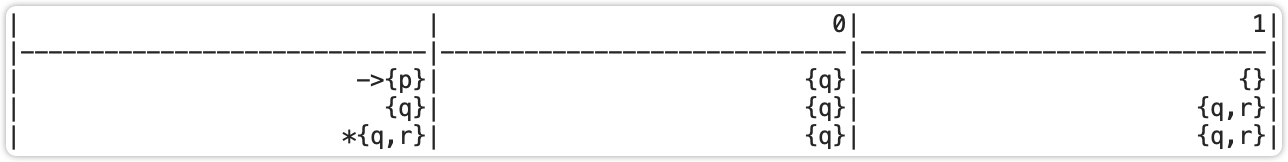
\includegraphics[width=\textwidth]{./Images/img1.png}

    \caption{样例输出\label{fig:img1}}

\end{figure}

\subsection{样例解释}

原NFA的转移表如\figref{fig:img2}。

\begin{figure}[htbp]

    \centering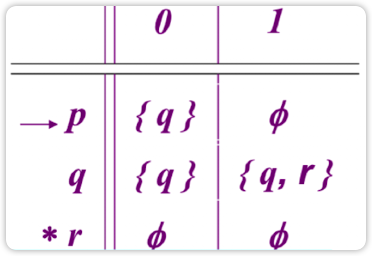
\includegraphics[width=0.4\textwidth]{./Images/img2.png}

    \caption{样例NFA的转移表\label{fig:img2}}


\end{figure}

\section{程序设计}

\subsection{环境}

\begin{itemize}
    \item macOS Big Sur 11.2.3
    \item gcc version 10.2.0
    \item C++11
\end{itemize}

\subsection{设计思路}

首先将状态和符号按照输入顺序从$0$开始编号,进而每一个状态集合都可以唯一对应一个二进制数。

以样例为例:状态$p,q,r$分别编号为$0,1,2$,符号$0,1$分别编号为$0,1$。则状态集合$\{p\}$可以表示为$001_2$即$1_{10}$,状态集合$\{q\}$可以表示为$010_2$即$2_{10}$,状态集合$\{q,r\}$可以表示为$110_2$即$6_{10}$。

在状态字符串和状态序号之间需要建立双向映射,分别用vector和unordered\_map实现。

进而NFA的状态转移可以用二维数组$delta$表示,其中第一维下标表示状态序号,第二维下标表示字符序号,数组的值表示状态集合对应的二进制数。

例如$delta[1][1]=6$表示序号为$1$的状态$q$通过序号为$1$的符号$1$转移到状态集合$\{q,r\}$。

通过子集构造法做等价转换,其过程无异于做深度优先搜索或者广度优先搜索,通过记录重复的状态,使得每个不同的状态最多遍历一次。而通过当前状态转移到下一个状态即对当前状态集合中每个元素的状态转移集合做并集,对于二进制数来说就是做或运算。

用二维数组$ans$表示DFA的状态转移表,其中每一行的第一个值存储原状态集合,其后的$m$个值依次为$m$种转移后的状态集合。

输出时,通过解析二进制数的每一位,依照映射输出对应的状态字符串。当出现初始状态和终止状态时加特殊标记,其中终止状态满足当前状态集合和原NFA的状态集合的交不为空集,即对应的二进制数做与运算不为$0$。

此外,程序通过求解$\varepsilon$-closure的方法,将$\varepsilon$-NFA转换成NFA。具体步骤参考代码注释。

\subsection{核心算法伪代码}

\begin{algorithm}[htbp]
    \caption{子集构造法\label{algo:cons}}
    \SetKwProg{Fn}{Function}{}{end}
    \SetKwData{Stat}{status}
    \SetKwData{NxtStat}{nextstatus}
    \SetKwData{Ans}{ans}
    \SetKwFunction{Dfs}{dfs}%
    \Fn(){\Dfs{\Stat}}{
    将\Stat 标记为已访问\;
    在\Ans 中增加新的一行,并将\Stat 记录为第一个元素\;
    \ForEach {符号$i$}
    {
        \NxtStat$\leftarrow 0$\;
        \ForEach {当前状态集合中的状态$j$}
            {\NxtStat $\leftarrow$\NxtStat$ \vee $状态$j$通过符号$i$转移到的状态集合\;}
        将\NxtStat 加入\Ans 的当前行\;
        \lIf{\NxtStat 没有访问过}{\Dfs{\NxtStat}}
    }
    }
\end{algorithm}

输入和输出的细节参考代码中的注释。通过设定PRINT\_WIDTH常量改变输出表格的宽度。

\section{调试分析}

\subsection{算法复杂度分析}

一般情况下,构建出的DFA与NFA的规模大体相当,所以算法的时间复杂度约为$O(n^2m)$,空间复杂度约为$O(nm)$。

在最坏情况下,算法需要遍历所有状态集合,此时时间复杂度为$O(2^nnm)$,空间复杂度为$O(2^nm)$。

\subsection{改进设想的经验和体会}

输入输出采用C++标准IO流,增加可读性。灵活应用C++标准库,节省编程复杂度和空间。

由于期望输出的$n$较小,范围假定在$64$之内,所以表示状态集合的数字用\mintinline{C++}{unsigned long long}类型。当$n$较大时程序可能很难在数秒的时间内运行完毕,并且此时需要用\mintinline{C++}{bitset}存储状态集合,但对时间复杂度和空间复杂度没有太大影响。

如果输入输出、数据结构采用常规C的方法,可能会有常数级别的优化,但是会大大增加编程复杂度。

由于NFA不合法的情况太多,难以一一判断,所以默认输入的是合法的NFA,没有做过多处理。

\section{测试结果}

\subsection{测试集1}

\subsubsection{输入}

\begin{listing}[H]
\begin{minted}{bash}
q0 q1 q2 q3
a b
q0 q1
q0
q2
q2
q3

q3
q3
q0
q3
\end{minted}
\end{listing}

\subsubsection{解释}

\begin{figure}[htbp]

    \centering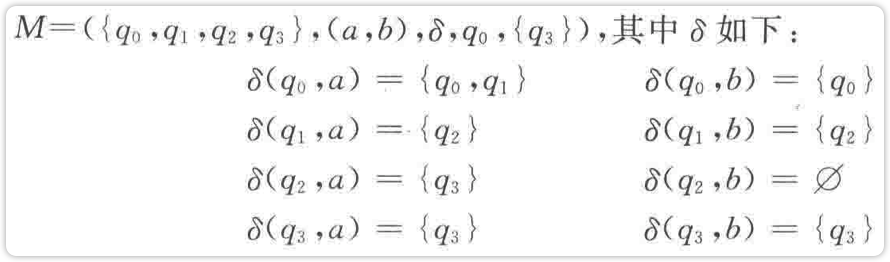
\includegraphics[width=0.6\textwidth]{./Images/img3.png}

\end{figure}

\subsubsection{输出}

\begin{figure}[htbp]

    \centering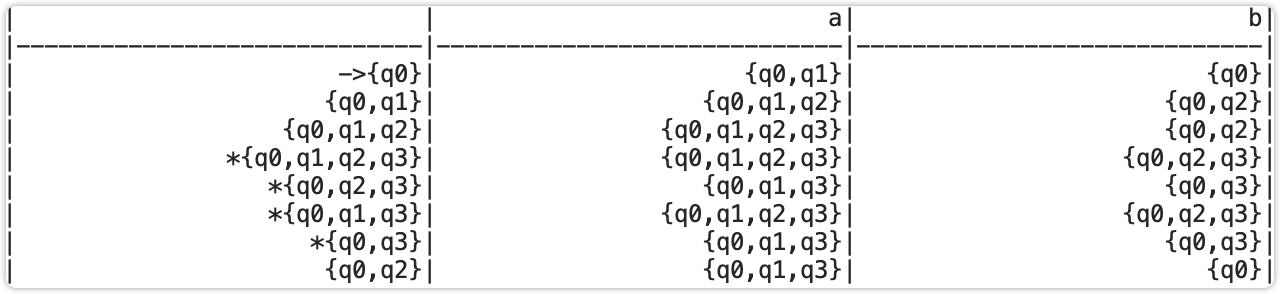
\includegraphics[width=\textwidth]{./Images/img4.png}

\end{figure}

\subsection{测试集2}

\subsubsection{输入}

\begin{listing}[H]
\begin{minted}{bash}
q0 q1 q2 q3 
a b
q1 q3
q1
q2
q1 q2
q3
q0

q0
q0
q1 q3
\end{minted}
\end{listing}

\subsubsection{解释}

\begin{figure}[htbp]

    \centering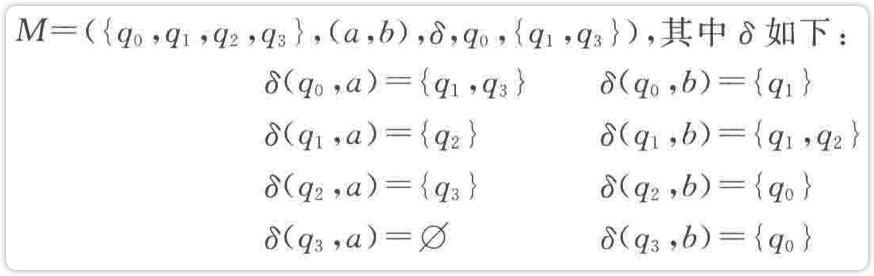
\includegraphics[width=0.6\textwidth]{./Images/img5.png}

\end{figure}

\subsubsection{输出}

\begin{figure}[htbp]

    \centering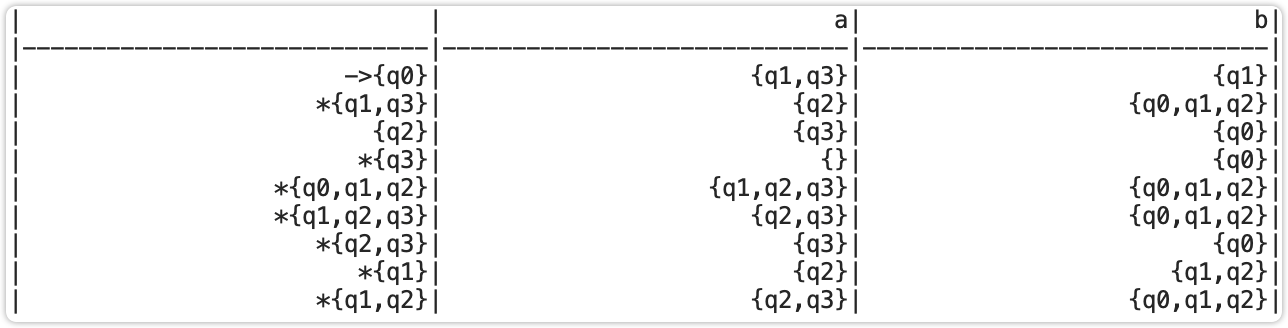
\includegraphics[width=\textwidth]{./Images/img6.png}

\end{figure}

\subsection{测试集3}

\subsubsection{输入}

\begin{listing}[H]
\begin{minted}{bash}
q0 q1 q2
0 1 2 [empty]
q0


q1

q1

q2


q2

q0
q2
\end{minted}
\end{listing}

\subsubsection{输出}

\begin{figure}[htbp]

    \centering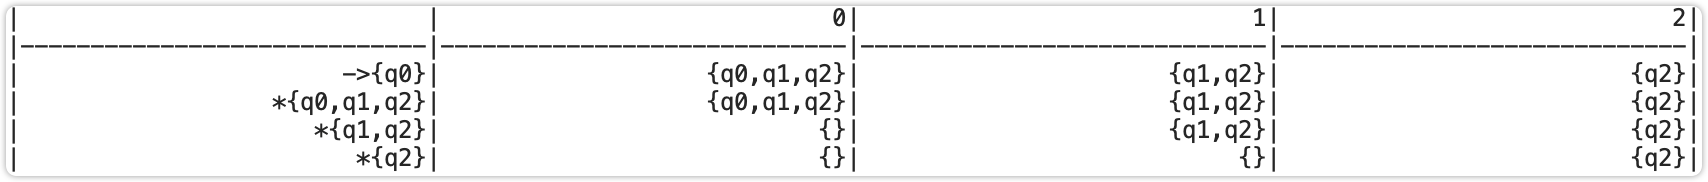
\includegraphics[width=\textwidth]{./Images/img7.png}

\end{figure}

\subsection{测试集4}

\subsubsection{输入}

\begin{listing}[H]
\begin{minted}{bash}
q0 q1 q2 q3 q4 q5
+ * 0 [empty]
q1
  

q1

q2
q1 q4



q3



q3
q5

q3






q0
q5
\end{minted}
\end{listing}

\subsubsection{解释}

\begin{figure}[htbp]

    \centering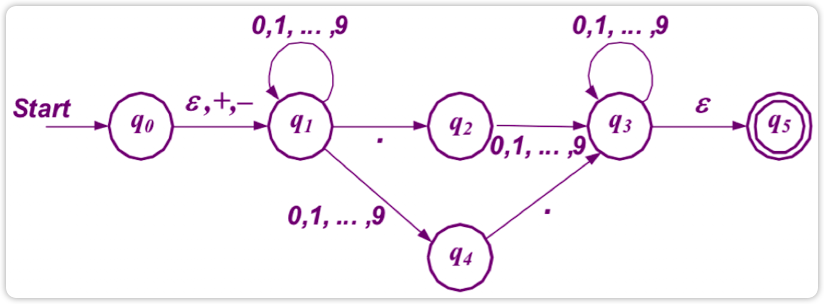
\includegraphics[width=0.6\textwidth]{./Images/img8.png}

\end{figure}

\subsubsection{输出}

\begin{figure}[htbp]

    \centering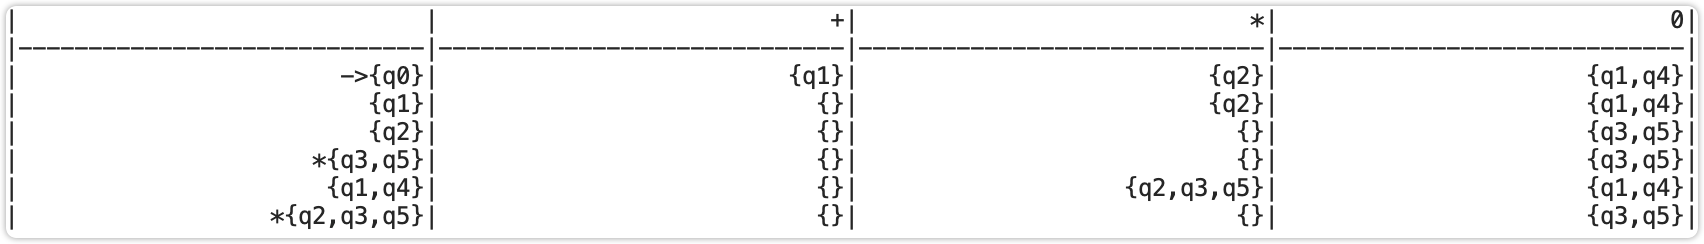
\includegraphics[width=\textwidth]{./Images/img9.png}

\end{figure}

\end{document}